\chapter{ Predicting optimal LMA distributions from environmental data using leaf photosynthesis models and whole plant hydraulics}

\section{Background}

%maybe an additional paragraph with a broade view of the research and its implications.

% First paragraph introduces the worldwide fast-slow spectrum, emphasizing how, despite the large diversity of species and phenotypes, functional trait variation is surprisingly low dimensional. Funnel intro leaf traits more specifically. 
Despite their extraordinary diversity, functional trait variation in terrestrial plants appears to be remarkably low dimensional \cite{diaz_global_2016}. The low-rank nature of plant functional traits is thought to emerge from physiological constraints common to all land plants. Furthermore, these constraints extend across various levels of plant performance, whereby multivariate correlations between traits give rise to a small number of axes that fully describe plant form and function \cite{reich2014a}. Nested within this space lies the well-known leaf economics spectrum (henceforth LES), which relates a number of leaf characteristics to the rate of return on investment into photosynthetic tissues \cite{wright2004a}. 

% More detail about the specific nature of leaf traits, how they are subdivided according to mass/area normalization
At its inception, the LES consisted of a single axis effectively quantifying the rate at which individual leaves recover the initial cost of constructing their respective tissues \cite{wright2004a}. Thus, the LES related 15 morphological and physiological characteristics of leaves to whether they offered a fast or slow return on investment. Subsequent studies demonstrated that some of the trait associations central to the LES were due to spurious correlations emerging from the mass normalization of specific traits \cite{osnas2013a}. The immediate implication was that several of the patterns observed in the mass-normalized LES were a consequence of the wide variation in LMA, coupled with the tight relationship between LMA and leaf lifespan (LL) \cite{osnas2013a}. Though this suggested the existence of traits orthogonal to the fast-slow spectrum, it cemented the veracity of the LMA-LL asymmetry, and highlighted the need for a mechanistic explanation.

Historically, the mechanisms underpinning the LES have been attributed to maximization of photosynthetic carbon assimilation throughout an individual leaf's lifespan \cite{wang2023a, kikuzawa_cost-benefit_1991}. While this view has provided some insight into the origins of certain traits (e.g., evergreeness vs. decidiousness), it does not adequately explain observed correlations between leaf traits and climate; this is best illustrated by the association between leaf mass per area (LMA) and aridity \cite{mitchell_leaf_2008}. An additional gap is the difficulty of linking carbon assimilation at the leaf level to whole-plant performance and fitness. 

%paragraph and figures with hypotheses and predictions


% A paragrpah on theoretical models that explain the origin of the LL-LMA association

%An additional paragraph hinting at hydraulics and scaling 

In an attempt to fill this gap, this chapter will use allometric scaling relationships to relate LMA and leaf lifespan to whole-plant carbon assimilation and water use. The principal question addressed is whether accounting for the effects of leaf characteristics on productivity and evapotranspiration at the organismal scale improves predictions of trait variation, compared to the single-leaf approach. In particular, I will focus on whether this novel approach can capture known correlations between leaf traits, body size, and aridity. Upon completion, this chapter will provide a link between leaf-level adaptations and organismal performance, adding to our understanding of the adaptive basis of leaf functional traits.

\section{Hypotheses and Predictions}

In this chapter I will be testing two main hypotheses. The leaf economics hypothesis, where LMA and LL are determined by optimal photosynthetic assimilation at the individual leaf level, and the hydraulic adjusted assimilation hypothesis in which LMA and LL are jointly constrained by plant-level hydraulics and optimal carbon assimilation. Each of these hypotheses predicts a specific value for both LMA and LL, as depicted in figure \ref{fig:pred}.

\begin{figure}[h!]
    \centering
    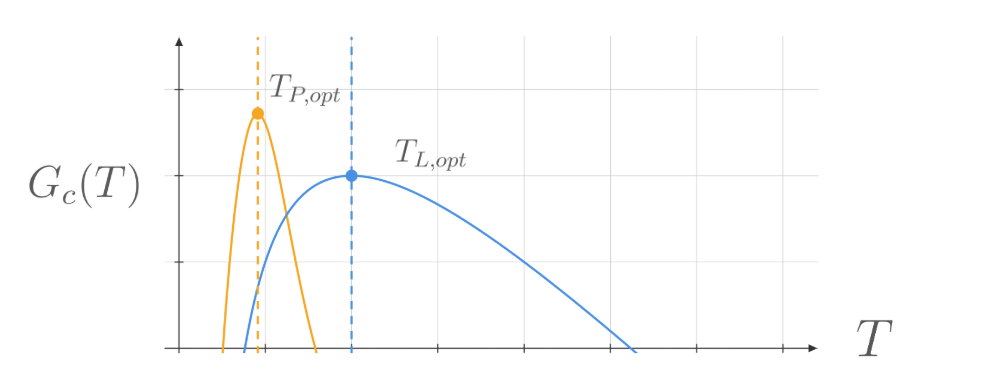
\includegraphics[width=0.95\textwidth]{figures/pred.png} 
    \caption{Optimal trait predictions under leaf economics (blue) and hydraulic-adjusted assimilation (orange) hypotheses. $G_c(T)$ is the assimilation rate as a function of a trait value $T$. $T_{P,opt}$ and $T_{L,opt}$ are the trait values where assimilation rate is maximized for the hydraulic-adjusted assimilation and leaf economics hypotheses respectively.}
    \label{fig:pred}
\end{figure} 

\section{Approach and Methods}

\subsection{Theory and modeling}
The first part of this chapter is a synthesis of trait-based models of single-leaf carbon assimilation with whole-plant growth and water use. Most of this initial phase has already been carried out, resulting in a simple framework that incorporates various leaf traits based on the general theory of leaf economics \cite{wang2023a, wang2017a, kikuzawa_cost-benefit_1991} along with allometric models of water use in trees \cite{kempes2011a}. The framework can be roughly separated into two distinct modules: (1) a biochemical model of single-leaf carbon assimilation and (2) allometric model of light interception, evapotranspiration, and water acquisition at the tree level. 

\subsubsection{Carbon assimilation}

At the leaf level, carbon assimilation is represented through a modified version of the model presented by Wang et al. \cite{wang2023a}, which is itself an extension of the Kikuzawa model \cite{kikuzawa_cost-benefit_1991}. Here, the instantaneous rate of carbon assimilation is represented as the sum of gross photosynthetic rate $A_{max}$, losses due to senescence ($B_{s}$), and construction costs ($C_c$).

\begin{equation}
    g(t) = A_{max}(1 - B_s(t)) - C_{c}(t)
\end{equation}

$A_{max}$ is the gross photosynthetic capacity, given average environmental conditions throughout the growing season. Senescence ($B_{s}$) is a time-dependent function and its progression follows a characteristic shape that is chiefly determined by LMA and the maximum rate of carboxylation \cite{xu_variations_2017}. 

\begin{equation}
    B_{s}(t) = \dfrac{t}{b}, \quad b = \dfrac{u LMA}{k_{1} k_{2} V_{cmax25}}
\end{equation}

Finally, $C_{c}$ is a time-varying function accounting for the carbon costs of constructing leaf tissues. The exact behavior of $C_{c}$ depends on leaf habit: deciduous trees make a single investment at the start of the growing season, whereas in evergreens construction costs accrue continuously. We estimate net carbon assimilation by averaging $g(t)$ throughout the year.

\begin{equation}
    \overline{g} =\dfrac{1}{365} \int_{s_{i}}^{s_{f}} A_{max}\left[1 - B_s(t)\right] - C_{c}(t) dt
\end{equation}

\subsubsection{Allometric scaling and hydraulics}

 Up to this point, carbon assimilation has been considered solely as a leaf-level phenomenon. Hereafter, we depart from previous analyses by integrating net assimilation across the canopy and incorporating whole-tree metabolism within the carbon budget. Canopy-wide carbon assimilation is treated further down, whereas losses due to metabolism are subtracted directly.

 \begin{equation}
    \overline{g} =\dfrac{1}{365} \left\{ A_{can}s_L\left[ 1 - \dfrac{s_L}{2b} \right] - \overline{C}_c\left(s_L, LMA, LL \right) - \beta_0 M^{\eta_0} \right\}
    \label{eq:net_g}
\end{equation}

Here, metabolism scales according to total tree biomass ($\beta_0M^{\eta_0}$) and annually averaged leaf construction costs are a function of growing season length $(s_L = s_f - s_i)$, LMA, and leaf longevity. In the case of deciduous trees, $\overline{C}_c$ is a single investment and is crucially determined by tree size, independent of either LL or LMA. The invariance of $\overline{C}_c$ with respect to LL and LMA in deciduous trees can be justified by noting that leaf longevity is constrained by $s_L$ and, given that photosynthetic biomass is necessarily proportional to total biomass \cite{niklas_invariant_2001}, LMA simply dictates how this biomass is allocated to leaf surface area.

To capture the relationship between leaf traits and climate, it is necessary to consider the effects of the environment on carbon assimilation as well as whole-tree water use. This, of course, requires a representation of canopy-wide energy budgets and light interception, as well as how the root system interfaces with soil moisture. This suite of processes is modeled after Kempes et al., \cite{kempes2011a}, including a few modifications which allow the integration of leaf traits, LMA in particular. Finally, the mathematical treatment of the biochemistry and physiology of photosynthesis is taken from the P-model \cite{stocker_p-model_2020}.

Having calculated the tree-wide rate of carbon assimilation and evapotranspiration, they can now be applied to equation \ref{eq:net_g}. The gross assimilation rate is substituted in $A_{can}$ directly, and the available flow rate of water ($Q_p$) is used to correct for potential water limitation. Water limitation is represented as a function of stomatal conductance $p(g_{ua})$, which is defined given a critical threshold $g_{crit}$:

\begin{equation}
    p(g_{ua}) = 
    \begin{cases}
         1 & \text{if $g_{ua} < g_{crit}$ }\\
         g_{ua}\omega/(g_{ua}g_{ul} - g_{ul}) & \text{otherwise}
    \end{cases}
\end{equation}

Here, $\omega$ subsumes the relationship between available evapotranspiration and the canopy's energy budget. As such, it is dependent on a suite of different functional traits, tree size, and climate. Further details of the model are omitted for brevity and are left for discussion elsewhere.


%paragraph on allometric model details (keep short, only essential details)


% Paragraph (and figures) presenting and interpreting preliminary results
Early simulations have shown that the model agrees qualitatively with the general trends leaf mass per area displays with climate variables, particularly with precipitation and temperature.

\begin{figure}[h!]
    \centering
    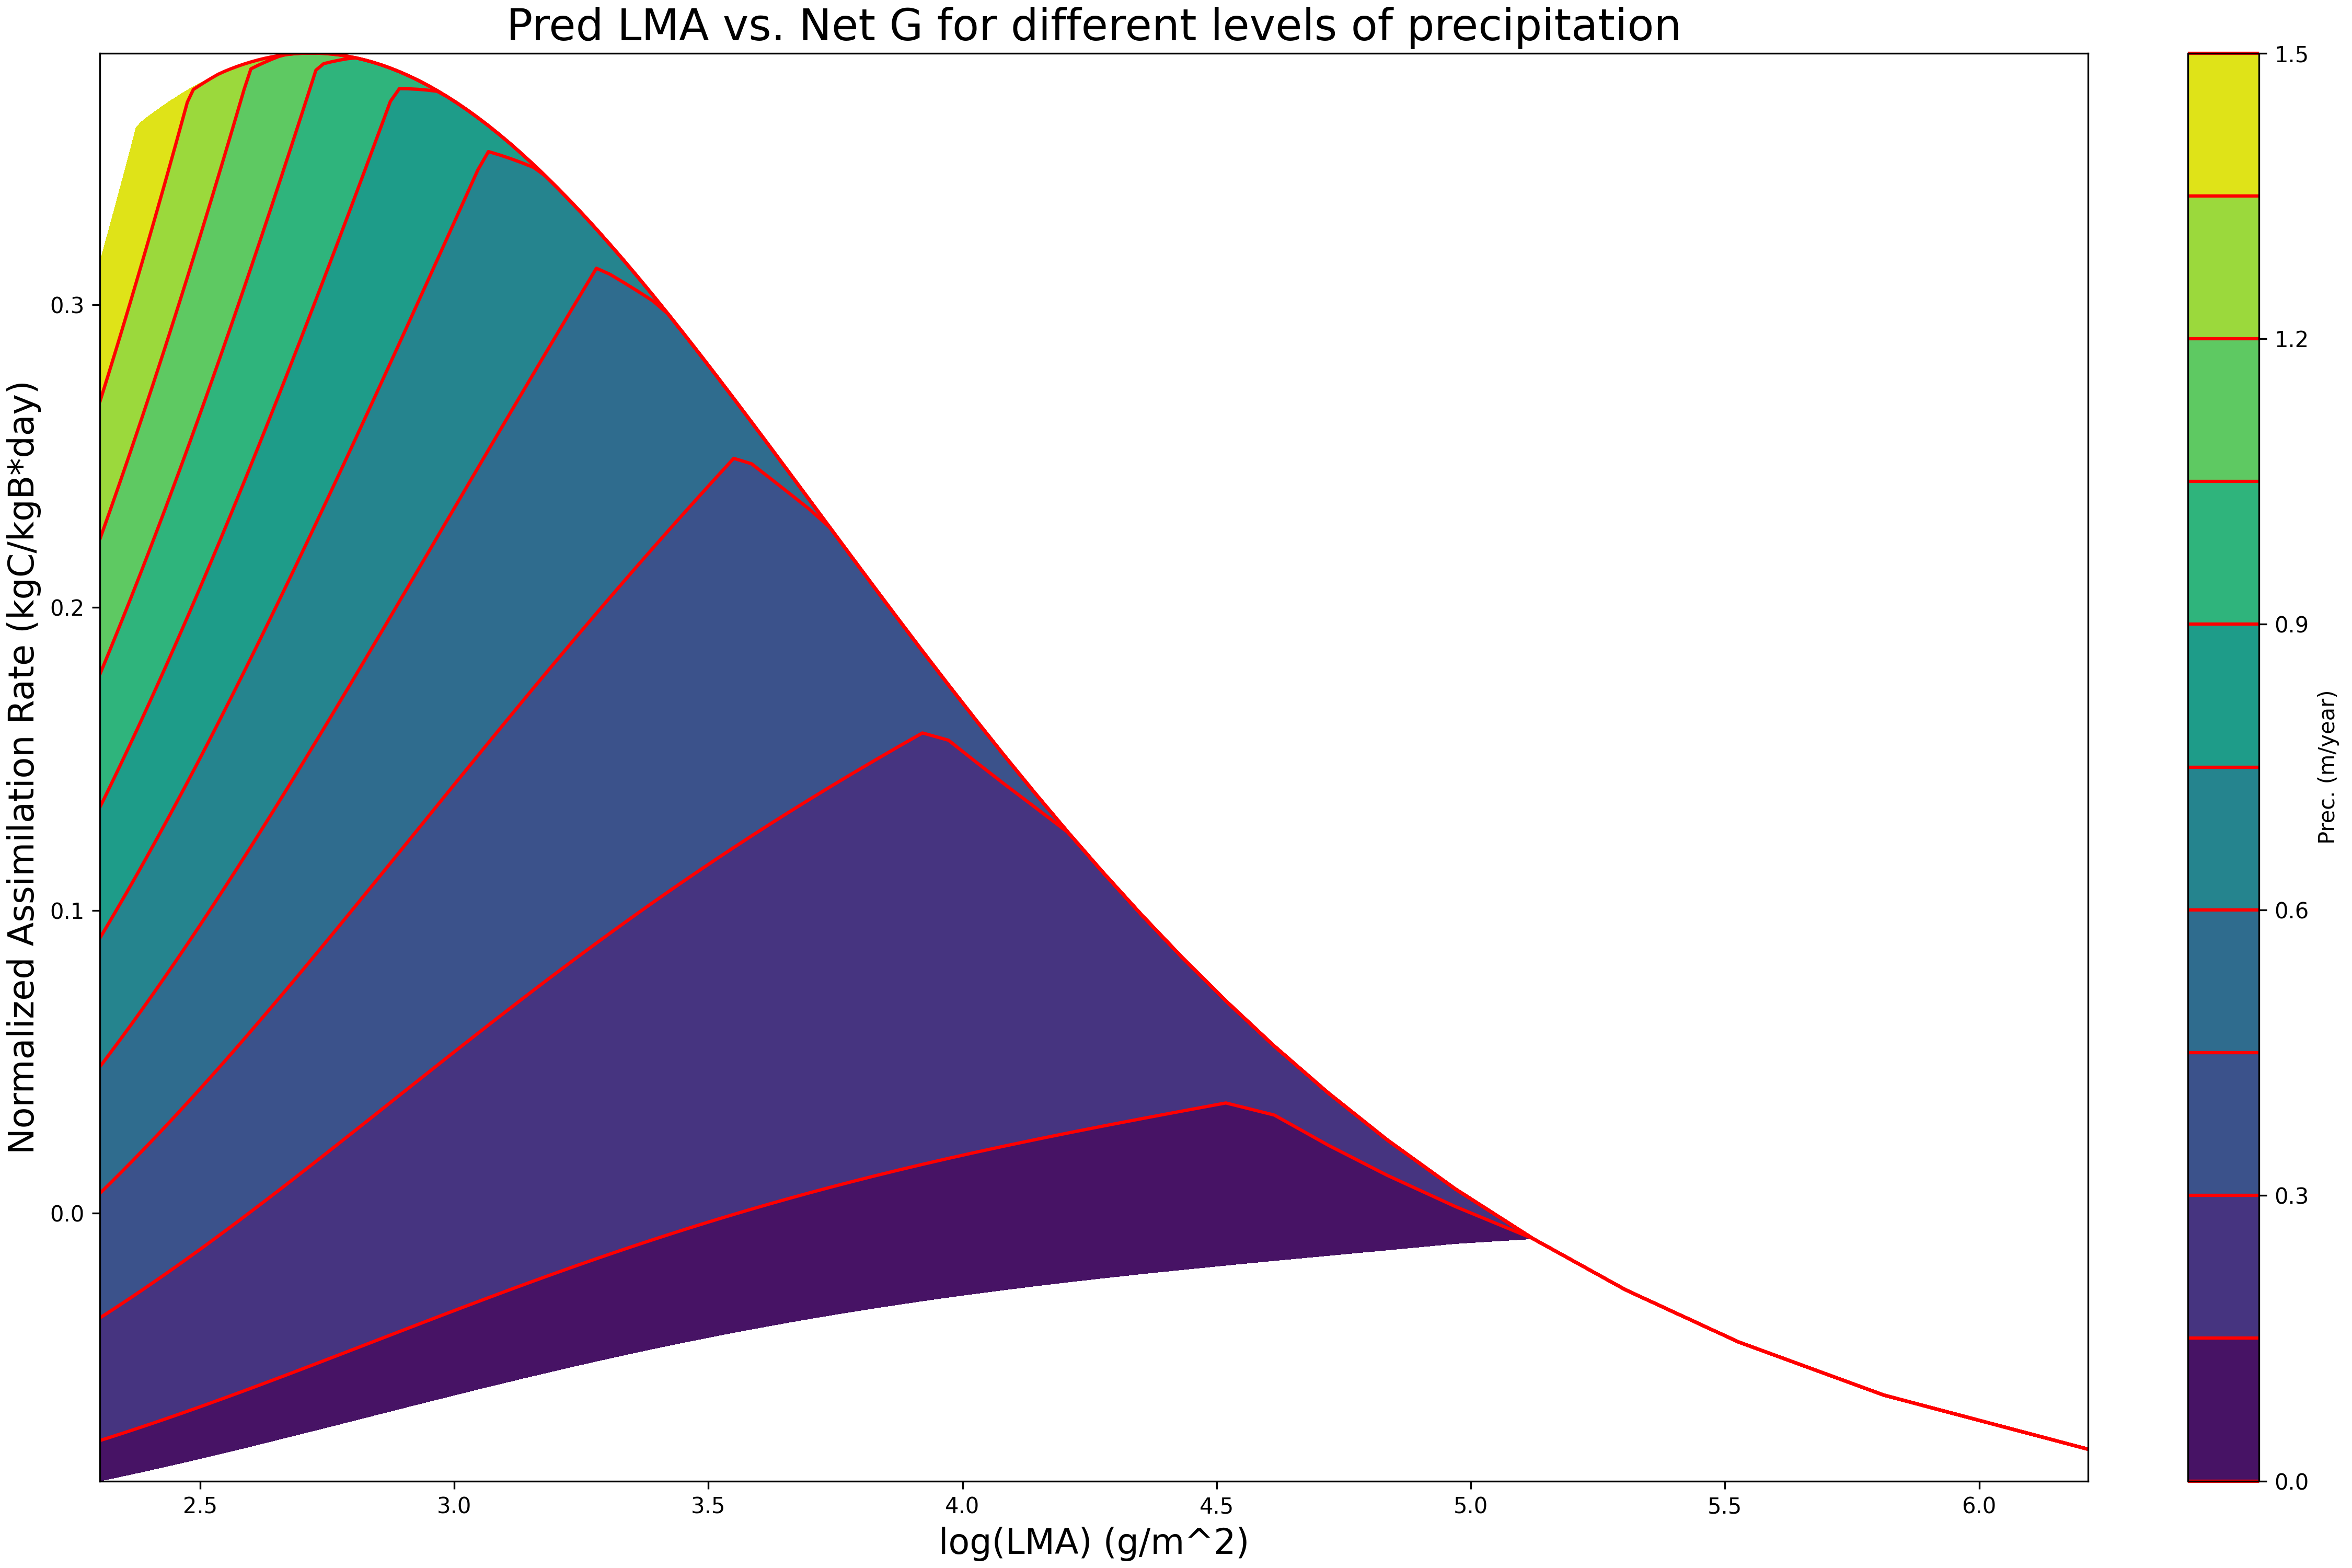
\includegraphics[width=0.95\textwidth]{figures/SLA_G_Pinc.png} 
    \caption{Normalized assimilation rate as a function of LMA and growing season precipitation. The simulations clearly show that the LMA at which assimilation rate is maximized shifts towards higher values as precipitation decreases which is consistent with observed global trends.}
    \label{fig:SLA_G_Pinc}
\end{figure} 

\subsection{Data and parameterization}
 
In order to make predictions it is necessary to parameterize and validate the model with empirical data. Fortunately, the model only has one free parameter, as all others are constrained through allometries or known physiological trade-offs. Validation will be carried out using trait data (cite data sources) containing abundance-weighted leaf mass per area moments, as well as the corresponding GPS coordinates. With the coordinates I will obtain the relevant climate variables through the CHELSEA geoclimatic models, along with estimated maximum tree heights found in the GEDI LIDAR database. A portion of the data will be used to parameterize stand water use efficiency, and the rest will be used to validate the model. 


% paragraph iving a detailed aount of data (variables, parameters, sources, other stuff)





